\begin{frame}{Librairie \texttt{keybert}}
\begin{itemize}[<+->]
\item extraction des mots/phrases-clés les plus similaires à un document
\item exploitation des plongements \textsc{BERT}\\
\hspace{-2cm}\item[\dangersign] la longueur des n-grammes à extraire n'est pas inférée en amont
\begin{itemize}[<+->]
\item \texttt{keyphrase\_ngram\_range=(1, 3)} : uni-, bi- ou trigrammes
\end{itemize}
\hspace{-2cm}\item[\dangersign] la grammaticalité des phrases n'est pas prise en compte \begin{itemize}
\item p. ex. \og{}scientifique les planches\fg{}
\end{itemize}
\end{itemize}
\end{frame}

\begin{frame}{Fonctionnement de la librairie \texttt{keybert}}
\begin{enumerate}[<+->]
\item entrée : un document
\item tokénisation du document en mots/phrases-clés candidates
\item génération des plongements du document et des mots/phrases-clés
\item calcul de la similarité cosinus document : mots/phrases-clés
\end{enumerate}
\begin{figure}
    \centering
    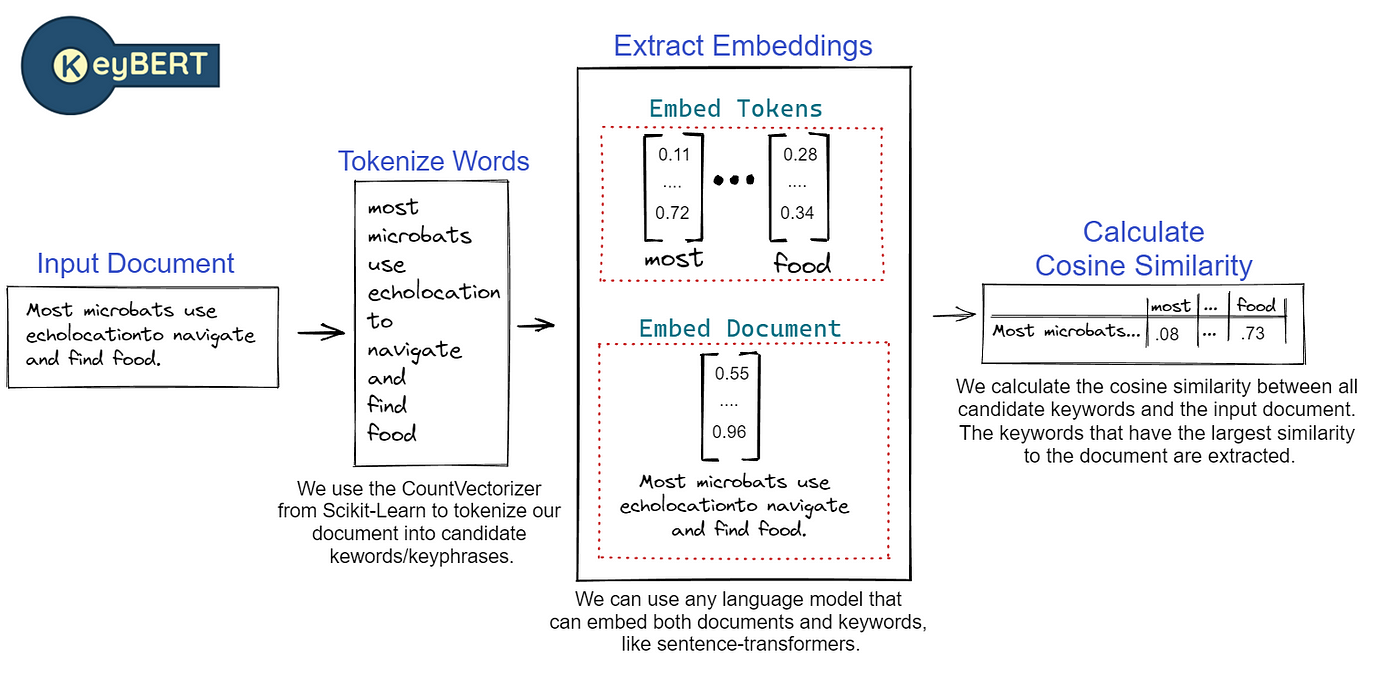
\includegraphics[width=80mm,scale=0.5]{pic/keybert.png}
    \caption{\textit{Pipeline} de la méthode \texttt{keybert} \citep{grootendorst2020keybert}.}
    \label{fig:enter-label}
\end{figure}
\end{frame}

\begin{frame}{\textit{Maximal Marginal Relevance} (\textit{\textsc{MMR}})}
\begin{itemize}[<+->]
\item paramètre de diversification des résultats
\item basé sur la similarité cosinus
\end{itemize}
\bigskip

\texttt{use\_mmr=True, diversity=[0-1]} \\
\hspace{2.77cm} {\footnotesize le degré de diversité entre 0 et 1}
\end{frame}

\begin{frame}{Liste des phrases-clés extraites avec \texttt{keybert}}
Liste des mots vides appliquées : \href{https://spacy.io/}{\texttt{spaCy}}
\begin{table}[!htb]
\footnotesize
    \begin{minipage}{.5\linewidth}
      \centering
        \begin{tabular}{l|r}
        \rowcolor[HTML]{FFCCC9} 
\textsc{\textbf{Phrase-clé}} & \cellcolor[HTML]{DAE8FC}\textsc{\textbf{Score}} \\ \hline
            scientifique planches reproduction & 0.5093 \\
			postérieure cordon postérieur & 0.5078 \\
			cervico dorsale & 0.465 \\
			sillon postérieur corne & 0.4644 \\
			région cervicale figure & 0.4572 \\
			cirrhose cancer primitif & 0.4355 \\
			altération cellules ganglionnaires & 0.4032 \\
			anatomie pathologique moëlle & 0.3931 \\
			lcucocythcs substance granuleuse & 0.3474 \\
			complètement détruite & 0.334
        \end{tabular}
        \subcaption{Corpus \og{}Charcot\fg{}.}
    \end{minipage}%
    \begin{minipage}{.5\linewidth}
            \begin{tabular}{||l|r}
        \rowcolor[HTML]{FFCCC9} 
\textsc{\textbf{Phrase-clé}} & \cellcolor[HTML]{DAE8FC}\textsc{\textbf{Score}} \\ \hline
     magnétisme applicable horticulture & 0.7012 \\
	droite corps envahie & 0.567 \\
	action nitrite amyle & 0.5114 \\
	trouve sabbat fans & 0.4422 \\
	centimètres rotule circonférence & 0.4194 \\ 
	mère attaques hystérie & 0.4148 \\
	chloral décembre règles & 0.4038 \\
	iconographie photographique salpetriere & 0.3977 \\
	poitrine apparent 11 & 0.3388 \\
	hystérogènes description attaques & 0.332
        \end{tabular}
        \subcaption{Corpus \og{}Autres\fg{}.}
      \centering
    \end{minipage}
    \caption{Liste de dix phrases-clés les plus pertinentes selon \texttt{keybert} dans les deux corpus.} 
\end{table}
%\begin{table}
%\small
%\begin{tabular}{l|r}
%\rowcolor[HTML]{FFCCC9} 
%\textsc{\textbf{Phrase-clé}} & \cellcolor[HTML]{DAE8FC}\textsc{\textbf{Score}} \\ \hline
%postérieure cordon postérieur & 0.5078 \\
%scientifique les planches &  0.4944 \\
%antérieure corne postérieure & 0.486 \\
%cervico dorsale & 0.465 \\
%cervicale la figure & 0.4311 \\
%faisceau postérieur tumeur & 0.4276 \\
%avoisinante cellule ganglionnaire & 0.3836 \\
%lcucocythcs substance granuleuse & 0.3474 \\
%moëlle épinière 45 & 0.3381 \\
%complètement détruite & 0.334 \\
%\end{tabular}
%\caption{Liste des dix phrases-clés les plus pertinentes selon \texttt{keybert}.}
%\end{table}
\end{frame}

